\documentclass[8pt,a4paper,compress]{beamer}

\usepackage{/home/siyer/lib/slides}

\title{Union-find}
\date{}

\begin{document}
\begin{frame}
\vfill
\titlepage
\end{frame}

\begin{frame}
\frametitle{Outline}
\tableofcontents
\end{frame}

\section{The Dynamic Connectivity Problem}
\begin{frame}[fragile]
\begin{minipage}{250pt}
\pause

Consider an input sequence of pairs of integers, where each integer represents an object of some type, and the pair $(p, q)$ means that ``$p$ is connected to $q$''

\pause
\bigskip

The goal of the dynamic connectivity problem is to devise a data structure to decide whether or not a new pair of objects is connected 

\pause
\bigskip

Applications
\begin{itemize}
\item Determine if two vertices in a network are connected

\item Determine if two variable names in a computer program are equivalent, ie, refer to the same object

\item If we think of the integers as belonging to mathematical sets, when we process a pair $(p, q)$, we are asking whether they belong to the same set, and if not, we unite $p$'s set and $q$'s set, putting them in the same set
\end{itemize}
\end{minipage}%
\begin{minipage}{60pt}
\hfill \visible<2->{\includegraphics[scale=0.35]{./figures/dyn_conn.pdf}}
\end{minipage}
\end{frame}

\begin{frame}[fragile]
\pause

We refer to the objects as sites, the pairs as connections, and the groups of connected sites as components

\pause
\bigskip

For simplicity, we assume that we have $N$ sites with integer names, from 0 to $N-1$

\pause
\bigskip

We solve the dynamic connectivity problem using the union-find data structure

\pause
\bigskip

The union-find (\lstinline{UF}) API
\begin{center}
\begin{tabular}{cc}
method & description \\ \hline
\lstinline$UF(int N)$ & \makecell{initialize an empty union-find data \\ structure with $N$ sites} \\
\lstinline$int find(int p)$ & component identifier for $p$ (0 to $N-1$) \\
\lstinline$int count()$ & number of components \\
\lstinline$boolean connected(int p, int q)$ & are $p$ and $q$ in the same component? \\
\lstinline$void union(int p, int q)$ & add connection between $p$ and $q$
\end{tabular} 
\end{center}
\end{frame}

\begin{frame}[fragile]
\begin{minipage}{250pt}

\pause
\smallskip

\lstinline{UF} client
\begin{lstlisting}[language=Java]
import edu.princeton.cs.algs4.QuickFindUF;
import edu.princeton.cs.algs4.StdIn;
import edu.princeton.cs.algs4.StdOut;

public class UFClient {
    public static void main(String[] args) {
        int N = StdIn.readInt();
        QuickFindUF uf = new QuickFindUF(N);
        while (!StdIn.isEmpty()) {
            int p = StdIn.readInt();
            int q = StdIn.readInt();
            if (uf.connected(p, q)) { continue; }
            uf.union(p, q);
            StdOut.println(p + " " + q);
        }
        StdOut.println(uf.count() + " components");
    }
}
\end{lstlisting}
    
\pause

\begin{lstlisting}[language={}]
$ more tinyUF.txt
10 4 3 3 8 6 5 9 4 2 1 8 9 5 0 7 2 6 1 1 0 6 7
\end{lstlisting}    

\pause

\begin{lstlisting}[language={}]
$ java UFClient < tinyUF.txt 
4 3
3 8
6 5
9 4
2 1
5 0
7 2
6 1
2 components
\end{lstlisting}
\end{minipage}%
\begin{minipage}{60pt}
\hfill \visible<2->{\includegraphics[scale=0.35]{./figures/dyn_conn.pdf}}
\end{minipage}
\end{frame}

\section{Quick Find}
\begin{frame}[fragile]
\pause

\begin{lstlisting}[language=Java]
package edu.princeton.cs.algs4;

public class QuickFindUF {
    private int[] id;
    private int count;

    public QuickFindUF(int N) {
        id = new int[N];
        count = N;
        for (int i = 0; i < N; i++) { id[i] = i; }
    }

    public int find(int p) { return id[p]; }

    public int count() { return count; }
  
    public boolean connected(int p, int q) { return id[p] == id[q]; }

    public void union(int p, int q) {
        int pID = id[p];
        int qID = id[q];
        if (pID == qID) { return; }
        for (int i = 0; i < id.length; i++) {
            if (id[i] == pID) { id[i] = qID; }
        }
        count--;
    }
}
\end{lstlisting}
\end{frame}

\begin{frame}[fragile]
\pause

Trace

\begin{center}
\visible<2->{\includegraphics[scale=0.7]{figures/quick_find_trace.pdf}}
\end{center}
\end{frame}

\section{Quick Union}
\begin{frame}[fragile]
\pause

\begin{lstlisting}[language=Java]
package edu.princeton.cs.algs4;

public class QuickUnionUF {
    private int[] parent;
    private int count;

    public QuickUnionUF(int N) {
        parent = new int[N];
        count = N;
        for (int i = 0; i < N; i++) { parent[i] = i; }
    }

    public int find(int p) {
        while (p != parent[p]) { p = parent[p]; }
        return p;
    }

    public int count() { return count; }
  
    public boolean connected(int p, int q) { return find(p) == find(q); }

    public void union(int p, int q) {
        int rootP = find(p);
        int rootQ = find(q);
        if (rootP == rootQ) { return; }
        parent[rootP] = rootQ; 
        count--;
    }
}
\end{lstlisting}
\end{frame}

\begin{frame}[fragile]
\pause

Trace

\begin{center}
\visible<2->{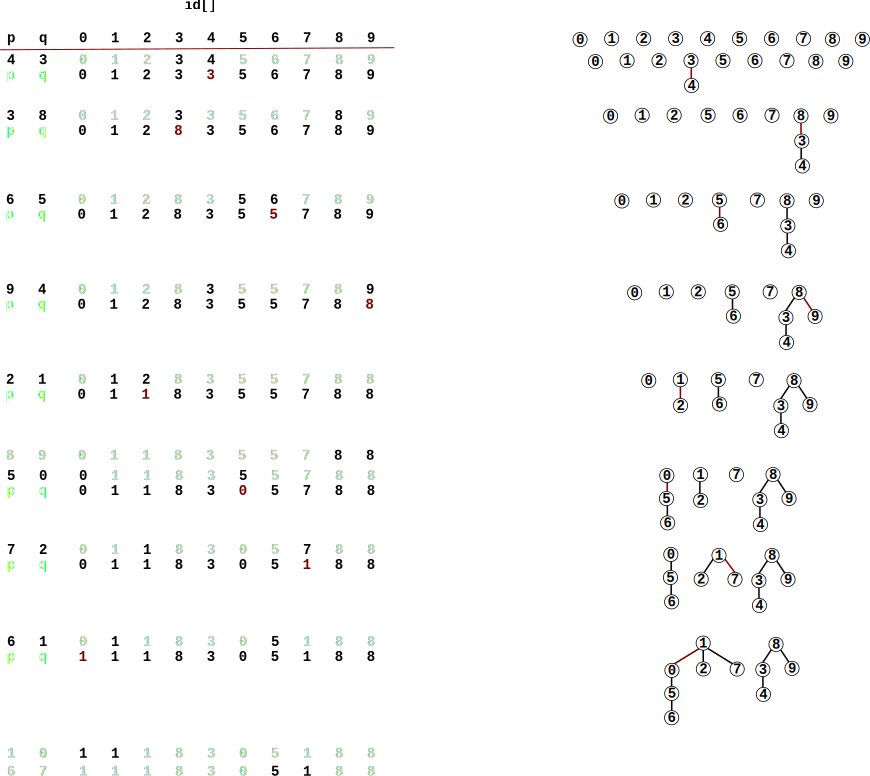
\includegraphics[scale=0.38]{figures/quick_union_trace.pdf}}
\end{center}
\end{frame}

\section{Weighted Quick Union}
\begin{frame}[fragile]
\pause

\begin{lstlisting}[language=Java]
package edu.princeton.cs.algs4;

public class WeightedQuickUnionUF {
    private int[] parent;
    private int[] size;
    private int count;

    public WeightedQuickUnionUF(int N) {
        parent = new int[N];
        size = new int[N];
        count = N;
        for (int i = 0; i < N; i++) { parent[i] = i; size[i] = 1; }
    }

    public int find(int p) {
        while (p != parent[p]) { p = parent[p]; }
        return p;
    }

    public int count() { return count; }
  
    public boolean connected(int p, int q) { return find(p) == find(q); }

    public void union(int p, int q) {
        int rootP = find(p), rootQ = find(q);
        if (rootP == rootQ) { return; }
        if (size[rootP] < size[rootQ]) {
            parent[rootP] = rootQ; size[rootQ] += size[rootP];
        }
        else {
            parent[rootQ] = rootP; size[rootP] += size[rootQ];
        }
        count--;
    }
}
\end{lstlisting}
\end{frame}

\begin{frame}[fragile]
\pause

Trace

\begin{center}
\visible<2->{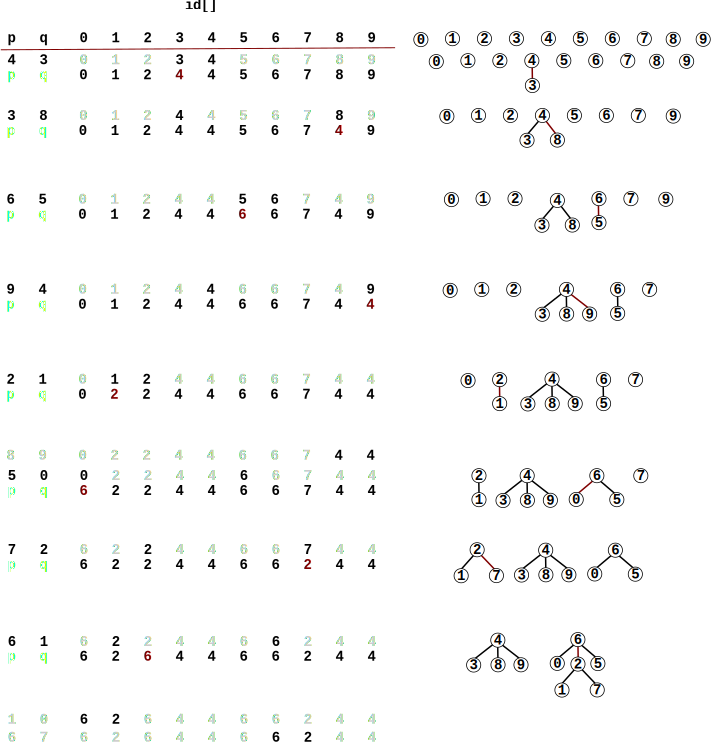
\includegraphics[scale=0.38]{figures/weighted_quick_union_trace.pdf}}
\end{center}
\end{frame}

\section{Performance Characteristics}
\begin{frame}[fragile]
\pause

Worst-case order of growth for $N$ sites
\begin{center}
\begin{tabular}{cccc}
data structure & constructor & union & find \\ \hline
quick-find & $N$ & $N$ & 1 \\
quick-union & $N$ & tree height & tree height \\
weighted quick-union & $N$ & $\log N$ & $\log N$ \\
\makecell{weighted quick-union \\ with path compression} & $N$ & $\approx 1$ (amortized) & $\approx 1$ (amortized) \\
impossible & $N$ & 1 & 1
\end{tabular} 
\end{center}
\end{frame}
\end{document}
